\lecture{11}{Индексирование гео.}
\subsection{Задачи поиска геометрии.}
\begin{itemize}
  \item Множество точек. Поиск точек, находящихся в прямоугольнике.
  \item Множество точек. Поиск ближайшей точки множества.
  \item Множество полигонов. Поиск полигонов множества, содержащих заданную точку.
  \item Множество полигонов. Поиск ближайшего полигона множества.
\end{itemize}

\subsection{kd-дерево}
\begin{figure}[H]    
  \centering    
  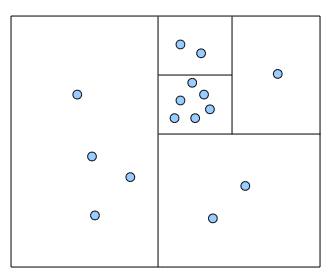
\includegraphics[width=0.5\textwidth]{figures/kdTree.png}    
  \caption*{Пример разбиения плоскости (каждое множество можно рассматривал как поддерево $k-d$ дерева)}   
\end{figure} 
\begin{definition}
  \highlight{K-d дерево} --- статическая структура данных для хранения точек в $k$-мерном пространстве.
  Позволяет отвечать на запросы, какие точки лежат в данном прямоугольнике. Каждое поддерево содержит
  некоторое множество точек. В поддереве точки разбиты три множества: точки левее, точки правее и 
  медиана (сам узел поддерева).
\end{definition}

Рассмотрим алгоритм построения:
\begin{enumerate}
  \item Разбиваем все точки вертикальной прямой на две примерно равных группы и получим правого и левого
    ребёнка
  \item Далее строим поддеревья для левого и правого ребёнка, но теперь уже разбиваем горизонтальной прямой
  \item На следующем уровне разбиваем снова вертикальными прямыми (или же, в случае больших размерностей
    разбиваем прямой, параллельной следующей оси координат)
  \item Продолжаем построение рекурсивно (окончание рекурсии, когда в поддереве оказывается одна вершина)
\end{enumerate}

\begin{figure}[H]    
  \centering    
  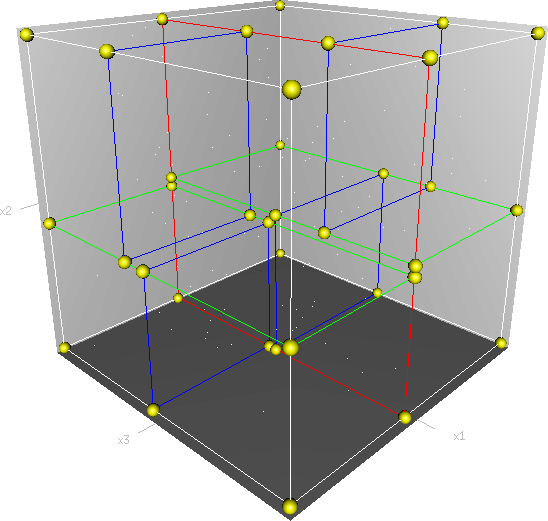
\includegraphics[width=0.5\textwidth]{figures/kdTree3D.png}    
  \caption*{Пример трёхмерного $k-d$ дерева}        
\end{figure} 

Возможная проблема такого разбиения: большое количество точек с одной координатой, в таком случае можно 
сравнивать лексиграфически (по нескольким координатам).

\begin{lemma}
  Данный алгоритм построения работает за $O(n \log n)$. 
\end{lemma}
\begin{proof}
  Напишем уравнение для рекурсии:
  \begin{gather*}
    T(n) = O(1), n = 1 \\
    T(n) = O(n) + 2 \cdot T\left( \frac{n}{2} \right)
  \end{gather*}
  По мастер-теореме о рекурсии получаем асимптотику $O(n \log n)$.
\end{proof}

\begin{figure}[H]    
  \centering    
  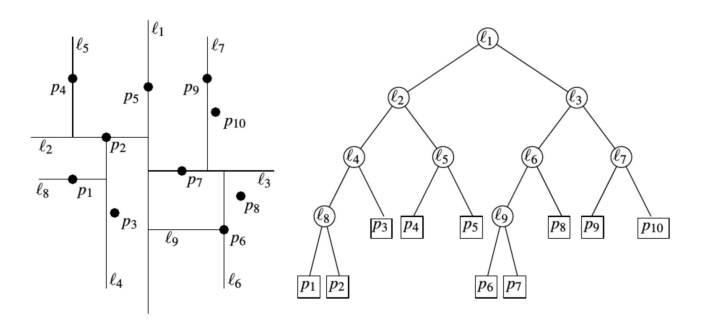
\includegraphics[width=0.8\textwidth]{figures/kdTreeConstruct.png}    
  \caption*{Ещё один пример $k-d$ дерева}        
\end{figure} 

Пусть  \texttt{region(V)} --- функция, которая возвращает по вершине область, за которую отвечает (её 
границы могут быть на бесконечности). Её можно считать при построении $k-d$ дерева или же вычислять
при поиске.

Опишем рекурсивный процесс поиска точек в прямоугольнике $R$ из вершины $V$ с детьми $V.left$ и 
$V.right$ соответственно (изначально $V = root$):
\begin{enumerate}
  \item Если $V$ --- лист, останавливаем процесс, возвращем все вершины из $V$ \item Если  \texttt{region(V.left)} $\subset R$, возвращаем $V.left$, 
    если же \texttt{region(V.left)} пересекает $R$, рекурсивно запускаем поиск от $V.left$
  \item Аналогично для правого ребёнка
\end{enumerate}

\begin{theorem}[О времени на запрос]
  Перечисление точек в прямоугольнике выполняется за $O(\sqrt{n} + ans)$, где $ans$ --- размер ответа.
\end{theorem}
\begin{proof}
  Нам необходимо оценить число рекурсивных вызовов (добавка $ans$ возникает, когда мы заканчиваем рекурсию).  
  Заметим, что рекурсивные вызовы выполняются только для тех вершин, регионы которых пересекают $R$, но
  не содержатся в нём. Такие регионы обязательно будут пересекать одну сторону хотя бы одну сторону $R$.
  Таким образом сведём задачу к оценки количества регионов, которые могут пересекаться, например, 
  произвольной вертикальной прямой. Обозначим как $Q(n)$ максимально возможное количество регионов,
  пересекаемых какой-либо вертикальной прямой в дереве.

  Рассмотрим произвольную вертикальную прямую, она будет пересекать регион корня и какого-то одного из
  его детей (пусть левого), но не будет пересекать регион другого ребёнка. Левый ребёнок разбит горизонтальной
  прямой на две части, в каждой примерно по $\frac{n}{4}$ вершин, причём эти части будут делиться также
  вертикальной прямой. Получаем рекурсивное соотношение:
  \begin{gather*}
    Q(n) = 2 + 2 \cdot Q \left( \frac{n}{4} \right) \\
    Q(n) = O(1), n = 1
  \end{gather*}
  Глубина дерева же:
  \[
    log_4 n = \frac{1}{2} \log_2 n
  .\] 
  Из мастер-теоремы получаем:
  \[
    Q(n) = O(2^{\frac{1}{2} \log_2 n}) = O(\sqrt{n})
  .\] 
  
\end{proof}

Кроме точек такие $k-d$ деревья можно строить для многоугольников.

\subsection{Гео-хеш.}
\begin{definition}
  \highlight{Гео-хеш} --- функция, которая преобразует точку на карте в строку. 
\end{definition}

Алгоритм разбиения Земли:
\begin{enumerate}
  \item Вся Земля разбивается на $32$ прямоугольника. $8$ по долготе, $4$ по широте.
  \item Каждый прямоугольник разбивается на $32$. $4$ по долготе, $8$ по широте.
  \item Каждый прямоугольник разбивается на $32$ прямоугольника. $8$ по долготе, $4$ по широте.
  \item $\ldots$
  \item Каждый из полученных прямоугольников обозначается символом из определённого алфавита.
\end{enumerate}

\begin{remark}
  Если представить каждый символ гео-хеша побитово, то чётные биты --- широта, нечётные --- долгота.
\end{remark}

Вычисление гео-хеша по точке:
\begin{enumerate}
  \item Координаты преобразуются из диапазонов $[-180, 180)$ и  $[-90, 90)$ в целые числа с нужной битностью
    (её можно вычислить по нужной длине гео-хеша)
  \item Сливаем биты широты и долготы по очереди
  \item Конвертируем в нужный алфавит (например, Base-32)
\end{enumerate}

\begin{remark}
  На основе гео-хешей можно строить различные хеш-таблицы для хранения геометрических объектов.
\end{remark}

